Город Брисбен был захвачен большими мутировавшими вомбатами, и вам требуется вывести людей в безопасное место.

Дороги в Брисбене организованы в виде большой решетки. Она представляет собой $R$ горизонтальных дорог, направленных с востока на запад и пронумерованных от $0$ до $R - 1$ с севера на юг. Аналогично, в Брисбене есть C вертикальных дорог, направленных с севера на юг и пронумерованных от $0$ до $C - 1$ с запада на восток,
как показано на рисунке ниже.

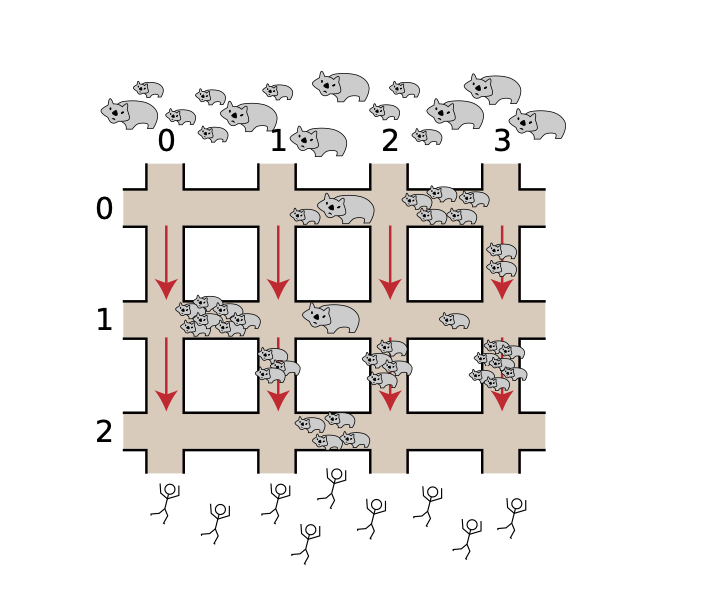
\includegraphics{wombats1.png}

Нашествие вомбатов началось с севера, и люди пытаются спастись на юге. Люди могут бежать по горизонтальным дорогам в любом направлении, однако по вертикальным дорогам они \textit{могут перемещаться только на юг}.

Перекресток горизонтальной дороги с номером $P$ и вертикальной дороги с номером $Q$ будем обозначать как $(P, Q)$. На каждом участке дороги между двумя перекрестками находится несколько вомбатов, и их количество может изменяться со временем. Ваша задача состоит в том, чтобы для человека, находящегося на каком­то конкретном перекрестке на самой северной дороге (горизонтальной дороге с номером $0$), указать такой путь до другого конкретного перекрестка на самой южной дороге (горизонтальной дороге с номером $R - 1$), на котором общее количество вомбатов будет минимально.

Изначально известны размеры дорожной решетки и количество вомбатов на каждом из участков дороги. После этого вам необходимо обработать серию из E событий, где каждое событие представляет собой одно из двух:
\begin{itemize}
\item либо изменяется количество вомбатов на каком­-либо участке дороги;
\item либо на некотором перекрестке на горизонтальной дороге с номером $0$ появляется человек, и вы должны найти путь от его местоположения до некоторого перекрестка на горизонтальной дороге с номером $R - 1$, на котором общее число вомбатов минимально.
\end{itemize}

Для обработки этих запросов вам необходимо реализовать функции \t{init()}, \t{changeH()}, \t{changeV()} и функцию \t{escape()} как описано ниже.

Ваше решение должно содержать функции \t{init()}, \t{changeH()}, \t{changeV()} и функцию \t{escape()}, которые должны быть описаны следующим образом:

Ваша функция \t{init()}:

\t{void init(int R, int C, int H[5000][200], int V[5000][200]);}

Эта функция задаёт изначальную ситуацию и позволяет инициализировать любые глобальные переменные и структуры данных. Она будет вызвана только один раз перед какими­либо другими вызовами функций \t{changeH()}, \t{changeV()} или \t{escape()}.

Параметры:
\begin{itemize}
\item $R$: количество горизонтальных дорог.
\item $C$: количество вертикальных дорог.
\item $H$: двумерный массив размера $R \cdot (C - 1)$, где $H[P][Q]$ задает количество вомбатов на участке горизонтальной дороги между перекрестками $(P, Q)$ и $(P, Q + 1)$.
\item $V$: двумерный массив размера $(R - 1) \cdot C$, где $V[P][Q]$ задает количество вомбатов на участке вертикальной дороги между перекрестками $(P, Q)$ и $(P + 1, Q)$.
\end{itemize}


Ваша функция \t{changeH()}:

\t{void changeH(int P, int Q, int W);}

Эта функция будет вызываться, когда изменяется число вомбатов на участке горизонтальной дороги между перекрёстками $(P, Q)$ и $(P, Q + 1)$.

Параметры:

\begin{itemize}
\item $P$: обозначает, на какой именно горизонтальной дороге расположен участок, на котором изменилось количество вомбатов $( 0 \leq P \leq R - 1 )$.
\item $Q$: обозначает, между какими именно двумя вертикальными дорогами находится участок дороги, на котором изменилось число вомбатов $( 0 \leq Q \leq C ­- 2 )$.
\item $W$: обозначает новое количество вомбатов на измененном участке дороги $( 0 \leq W \leq 1 000 )$.
\end{itemize}


Ваша функция \t{changeV()}:

\t{void changeV(int P, int Q, int W);}        


Эта функция будет вызываться, когда изменяется число вомбатов на участке вертикальной дороги между перекрёстками $(P, Q)$ и $(P + 1, Q)$.

Параметры:
\begin{itemize}
\item $P$: обозначает, между какими именно двумя горизонтальными дорогами находится участок дороги, на котором изменилось число вомбатов $( 0 \leq P \leq R -­ 2 )$
\item $Q$: обозначает, на какой именно вертикальной дороге расположен участок, на котором изменилось количество вомбатов $( 0 \leq Q \leq C - 1 )$.
\item $W$: обозначает новое количество вомбатов на измененном участке дороги $( 0 \leq W \leq 1 000 )$.
\end{itemize}



Ваша функция \t{escape()}:

\t{int escape(int V1, int V2);}


Эта функция должна вычислять минимальное возможное количество вомбатов, которое может встретить человек на пути от перекрёстка $(0, V1)$ до перекрестка
$(R - 1, V2)$. 

Параметры:
\begin{itemize}
\item $V1$: обозначает, где именно человек изначально находится на горизонтальной дороге с номером $0$ $( 0 \leq V1 \leq C - 1 )$.
\item $V2$: обозначает, где именно человек должен закончить свой путь на горизонтальнойдорогесномером $R­-1$ $(0\leq V2\leq C­1)$.
\item \textit{Возвращаемое значение}: минимальное количество вомбатов, которое человек может встретить на пути от одного перекрестка до другого.
\end{itemize}
